\section{Elementary Perceptual Tasks}

Cleveland and McGill describe the mapping of graphical elements to quantitative variables as \emph{elementary perceptual tasks} and introduce a list of ten different encodings in their paper~\cite{cleveland_mcgill}. We create visualizations of these tasks as rasterized images (Fig.~\ref{fig:elementary_perceptual_tasks}).

\subsection{Parametrizations}
\label{sec:parametrizations}
We generate multiple parameterizations for each elementary perceptual task (Fig.~\ref{fig:elementary_perceptual_tasks}) and sequentially increase the number of parameters. For instance, for \emph{position non-aligned scale} we first only vary the origin of the coordinate system which yields just 10 different parameters. We then include translation along the y-axis with a significant increase in variability. We then also add x-movement and a variable spot size. This results in more complex datasets depending on the variability setting. Table~\ref{tab:encoding_parameters} shows the different settings. It is important to consider this variability when evaluating different classifiers with individual trainable parameters (Table~\ref{tab:parameters}).

\begin{figure}[t]
	  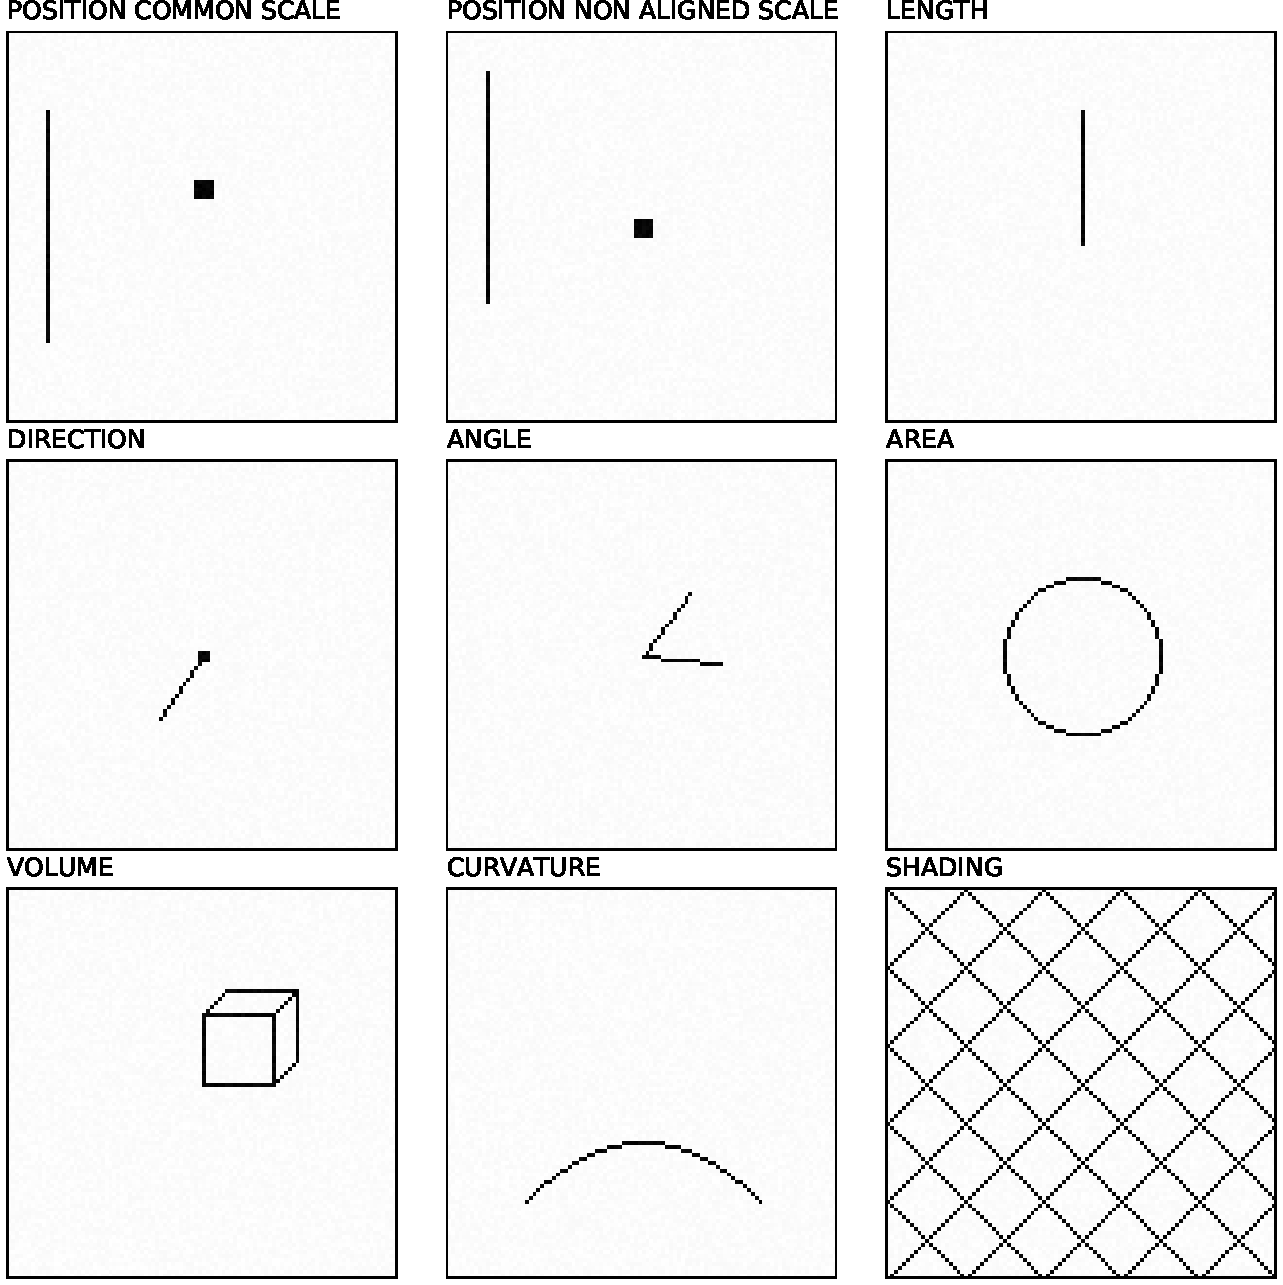
\includegraphics[width=\linewidth]{figure1_overview.pdf}
  \caption{\textbf{Elementary Perceptual Tasks.} Rasterized visualizations of the elementary perceptual tasks as defined by Cleveland and McGill~\cite{cleveland_mcgill} (color saturation excluded). We vary the parameters of each perceptual task and then assess the interpretability of feed-forward neural networks.}
	\label{fig:elementary_perceptual_tasks}
\end{figure}

\begin{table}[t]
\centering
\caption{\textbf{Variability of Elementary Perceptual Tasks.} We sequentially increase the number of parameters for every visual encoding of the elementary perceptual tasks. This introduces variability and increasingly more complex datasets.}
\resizebox{\linewidth}{!}{
\begin{tabular}{llr}
%	\toprule
%	\makecell{Classifier} & \makecell{Convolutional\\Layers} & \makecell{Trainable\\Parameters} \\
%	\midrule
%	MLP & $0$ & $2,560,513$ \\
%	\emph{LeNet} + MLP & $2$ & $8,026,083$ \\
%	\emph{VGG19} + MLP & $16$ & $21,204,545$ \\
%	\emph{Xception} + MLP & $36$ & $25,580,585$ \\
%	\bottomrule
	\toprule
	Elementary Perceptual Task & Variability & Parameters\\
	\midrule
	\makecell[tl]{\emph{Position Common Scale}} & \makecell[tl]{Position Y\\+ Position X \\+ Spot Size \\} & \makecell[tr]{ $60$ \\ $3600$ \\ $21600$}\\

	\midrule
	\makecell[tl]{\emph{Position Non-Aligned Scale}} & \makecell[tl]{Position Y\\+ Position X \\+ Spot Size \\} & \makecell[tr]{ $600$ \\ $36000$ \\ $216000$}\\

	\midrule
	\makecell[tl]{\emph{Length}} & \makecell[tl]{Length\\+ Position Y \\+ Position X \\+ Width} & \makecell[tr]{ $60$ \\ $2400$ \\ $144000$\\$864000$}\\

	\midrule
	\makecell[tl]{\emph{Direction}} & \makecell[tl]{Angle\\+ Position Y \\+ Position X} & \makecell[tr]{ $360$ \\ $21600$ \\ $1296000$}\\

	\midrule
	\makecell[tl]{\emph{Angle}} & \makecell[tl]{Angle\\+ Position Y \\+ Position X} & \makecell[tr]{ $90$ \\ $5400$ \\ $324000$}\\

	\midrule
	\makecell[tl]{\emph{Area}} & \makecell[tl]{Radius\\+ Position Y \\+ Position X} & \makecell[tr]{ $40$ \\ $800$ \\ $16000$}\\

	\midrule
	\makecell[tl]{\emph{Volume}} & \makecell[tl]{Cube Sidelength\\+ Position Y \\+ Position X} & \makecell[tr]{ $20$ \\ $400$ \\ $8000$}\\
	
	\midrule
	\makecell[tl]{\emph{Curvature}} & \makecell[tl]{Midpoint Curvature\\+ Position Y \\+ Position X} & \makecell[tr]{ $80$ \\ $1600$ \\ $64000$}\\	

	\midrule
	\makecell[tl]{\emph{Shading}} & \makecell[tl]{Density\\+ Position Y \\+ Position X} & \makecell[tr]{ $100$ \\ $2000$ \\ $40000$}\\	
	
	\bottomrule
\end{tabular}
}
\label{tab:encoding_parameters}
\end{table}

\subsection{Hypotheses}

We proposed four hypotheses entering the elementary perceptual task experiment:

\begin{itemize}
	\item \textbf{H1.1} \textbf{Visual cortex inspired classifiers are able to connect graphical elements to their quantitative variables.} While much simpler models than their biological pendant, convolutional neural networks are heavily influenced by our biological knowledge of the visual system. Such classifiers therefor follow the same principles as human perception.
	\item \textbf{H1.2} \textbf{Computed perceptual performance is dependent on classifier complexity.} We evaluate multiple classifiers with different numbers of trainable parameters. A more complex classifier (with higher number of parameters) will perform better on elementary perceptual tasks.
	\item \textbf{H1.3} \textbf{Some visual encodings are better than others for computations.} Cleveland and McGill order the elementary perceptual tasks by accuracy. We investigate whether this order is also relevant for computing graphical perception.
	\item \textbf{H1.4} \textbf{Classifiers trained on perceptual tasks can generalize to more or less complex variations of the same task.} Recent research suggests that convolutional neural networks generalize extremely well. While the underlying reasons are mainly yet unknown, this property allows them to perform on variations of a similar perceptual task.
\end{itemize}
